\begin{samplecase}
{\bf Fission cross sections: n + ${}^{232}$Th}\newline
It is well known that a systematic approach for fission is difficult to achieve.
It is possible to obtain
very satisfactory fits to fission data with TALYS, but at the expense of using
many adjustable input parameters.
We are performing extensive model calculations to bring somewhat more structure
in the collection of fitting parameters. In the meantime, we include here a
sample case for the description of the fission cross section of $^{232}$Th.
We use the following input file,

\VerbatimInput{\samples n-Th232-fis/org/talys.inp}

Note that, although no adjustable parameters are visible above,
this is certainly no ``default'' calculation.
Instead, this sample case illustrates the use of so-called ``best files''.
By using the {\bf best y} keyword, the file
{\em talys/structure/best/Th232/n-Th232.talys} is automatically invoked.
The contents of that file are

\VerbatimInput{/Users/koning/talys/structure/best/Th232/n-Th232.talys}

The above parameters are the usual ones to be adjusted to get good
agreement with experimental data: level density and fission parameters for
the ground state or on top of the barriers.
The resulting file {\em fission.tot} is plotted
together with experimental data in Fig.~\ref{fissioneps}.

Due to the presence of {\bf outfission y} in the input file, all nuclear
structure related to the fission process is given in the output for the target
and the compound nucleus
{\small \begin{verbatim}

 Fission information for Z= 90 N=142 (232Th)

 Number of fission barriers           :  2
 Number of sets of class2 states      :  1

 Parameters for fission barrier  1

 Type of axiality                     :  1
 Height of fission barrier 1          :   5.800
 Width of fission barrier 1           :   0.900
 Rtransmom                            :   0.600
 Moment of inertia                    :  87.657
 Number of head band transition states:  8
 Start of continuum energy            :   0.800

 Head band transition states

  no.    E    spin    parity

    1   0.000   0.0   +
    2   0.500   2.0   +
    3   0.400   0.0   -
    4   0.400   1.0   -
    5   0.500   2.0   +
    6   0.400   2.0   -
    7   0.800   0.0   +
    8   0.800   0.0   +

Rotational bands

  no.    E    spin    parity

    1   0.000   0.0   +
    2   0.034   2.0   +
    3   0.114   4.0   +
    4   0.240   6.0   +
    5   0.400   1.0   -
    6   0.400   2.0   -
    7   0.411   8.0   +
    8   0.411   1.0   -
    9   0.423   2.0   -
   10   0.434   3.0   -
..................
Parameters for fission barrier  2

 Type of axiality                     :  2
 Height of fission barrier 2          :   6.318
 Width of fission barrier 2           :   0.600
 Rtransmom                            :   1.000
 Moment of inertia                    : 154.212
 Number of head band transition states:  4
 Start of continuum energy            :   0.500

 Head band transition states

  no.    E    spin    parity

    1   0.000   0.0   +
    2   0.500   2.0   +
    3   0.200   0.0   -
    4   0.500   1.0   -
.............
\end{verbatim} } \renewcommand{\baselinestretch}{1.07}\small\normalsize
\noindent

Moreover, the corresponding fission transmission coefficients are printed for
all excitation energies encountered in the calculation
{\small \begin{verbatim}

 Fission transmission coefficients for Z= 90 N=143 (233Th) and an excitation en

   J      T(J,-)      T(J,+)

  0.5   4.02053E-08 6.51894E-08
  1.5   0.00000E+00 0.00000E+00
.............
\end{verbatim} } \renewcommand{\baselinestretch}{1.07}\small\normalsize
The fission information for all residual nuclides can be obtained in the
output file as well by adding {\em outpopulation y} to the input file.

As an exercise, the user may want to try to adjust the first fission barrier
of $^{232}$Th to get a better fit of the second chance fission cross section.

\end{samplecase}
\begin{figure}
\centering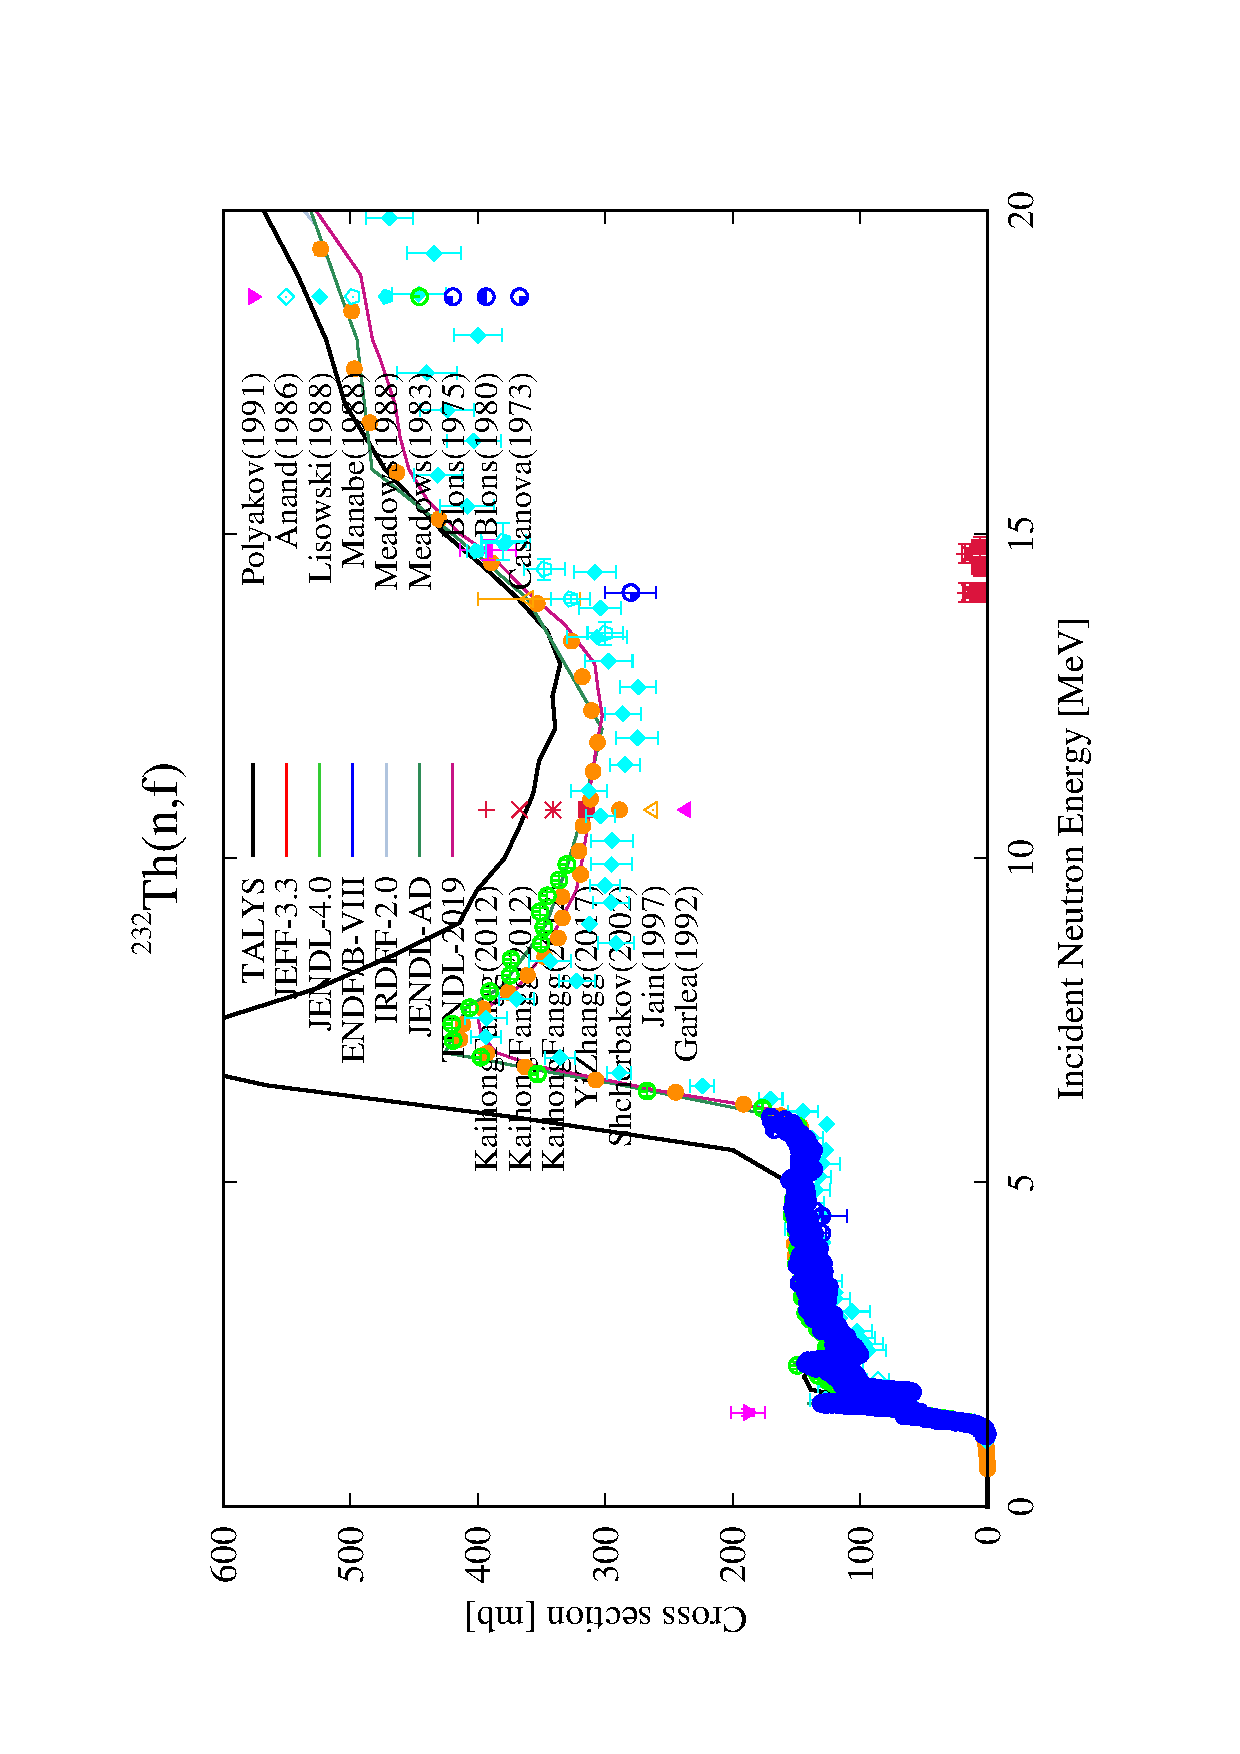
\includegraphics[scale=0.5,angle=270]{n-Th232-fis}
\caption{Neutron induced fission cross section of ${}^{232}$Th compared with
experimental data.}
\label{fissioneps}
\end{figure}
